\documentclass[journal,12pt,onecolumn,draftclsnofoot]{IEEEtran}  % Comment this line out
                                                          % if you need a4paper
% \documentclass[a4paper, 10pt, conference]{ieeeconf}      % Use this line for a4
                                                          % paper
\IEEEcompsocthanksitem
\IEEEoverridecommandlockouts                              % This command is only
                                                          % needed if you want to
                                                          % use the \thanks command
% \overrideIEEEmargins
% See the \addtolength command later in the file to balance the column lengths
% on the last page of the document

\usepackage{subcaption}
% \captionsetup{compatibility=false}
% The following packages can be found on http:\\www.ctan.org
\usepackage{graphics} % for pdf, bitmapped graphics files
%\usepackage{epsfig} % for postscript graphics files
%\usepackage{mathptmx} % assumes new font selection scheme installed
%\usepackage{times} % assumes new font selection scheme installed
\usepackage{amsmath} % assumes amsmath package installed
%\usepackage{amssymb}  % assumes amsmath package installed
\usepackage{balance}
\usepackage[font=small,labelfont=bf]{caption} % makes figure captions small, and figure labels bold
\usepackage{tikz}
\usetikzlibrary{calc}
\usepackage[autostyle]{csquotes}  %makes block quotes possible
\usepackage{float} %insures proper placement of figures

\title{Classifying Brain States Using Causal Brain Networks}


\author{Kamal Kamalaldin}

\usepackage{neuralnetwork}
\begin{document}

\maketitle

\section{Definition}
\subsection{Project Overview}
This project explores the possibility applications of unsupervised learning on classifying different brain states in a rat's brain. The topic is in the neuroscience field, and the motivation behind this project is to help detect epilepsy in the human brain. Although there have been approaches to solving this problem by applying neural networks to EEG signals, and a recent competition has been launched on Kaggle that deals with epilepsy prediction, we take a different approach to this problem by relying on a causality model that is not often used in the field of machine learning. This causality model, Sugihara Causality, is used as a means to establish a measure of brain communication patterns. Using this causality model, we were able to build a series of graphs each of which (theoretically) represents a snapshot of brain communication. Since these graphs are highly dimensional, we use PCA to attempt to reduce its complexity before clustering. we then analyze different clustering possibilities and finally observe if clustering gives an intelligible insight into classifying epileptic and non epileptic brain states. 


The dataset used in this project has been collected privately by Dr. Zsolt Borhegyi at MTA-TKI , MTA-ELTE-NAP B-Opto-Neuropharmacology Group in Hungary. The original data consisted of EEG recordings of a rat's brain. The processed (graph series) version of the data can be downloaded from https://drive.google.com/file/d/0BzyCB-i-aKDWU2pBYkVoOV81S3M/view?usp=sharing. The research conducted in this paper was also funded by the NSF as part of grant $1359275$ at the University of Colorado Colorado Springs. 

\subsection{Methods}
\subsubsection{Data Collection}
EEG data was collected from an 4x8 endodermal electrode array at a frequency of 1000 Hz (31 channels, one channel malfunctioned, Fig. \ref{fig:rat_experiment}). The data recording lasts for ~500 seconds, during which epileptic seizures were evoked using 4-aminopyridine and EEG data was recorded from the electrode array. The spiking voltage of each recorded electrode is used as a signal and is referred to as a channel (Fig. \ref{fig:example_eeg_and_kcsd}). Each channel has a continuous data series that spans the 500 seconds.

\begin{figure}[H]
  \centering
  \begin{subfigure}[b]{0.45\textwidth}
    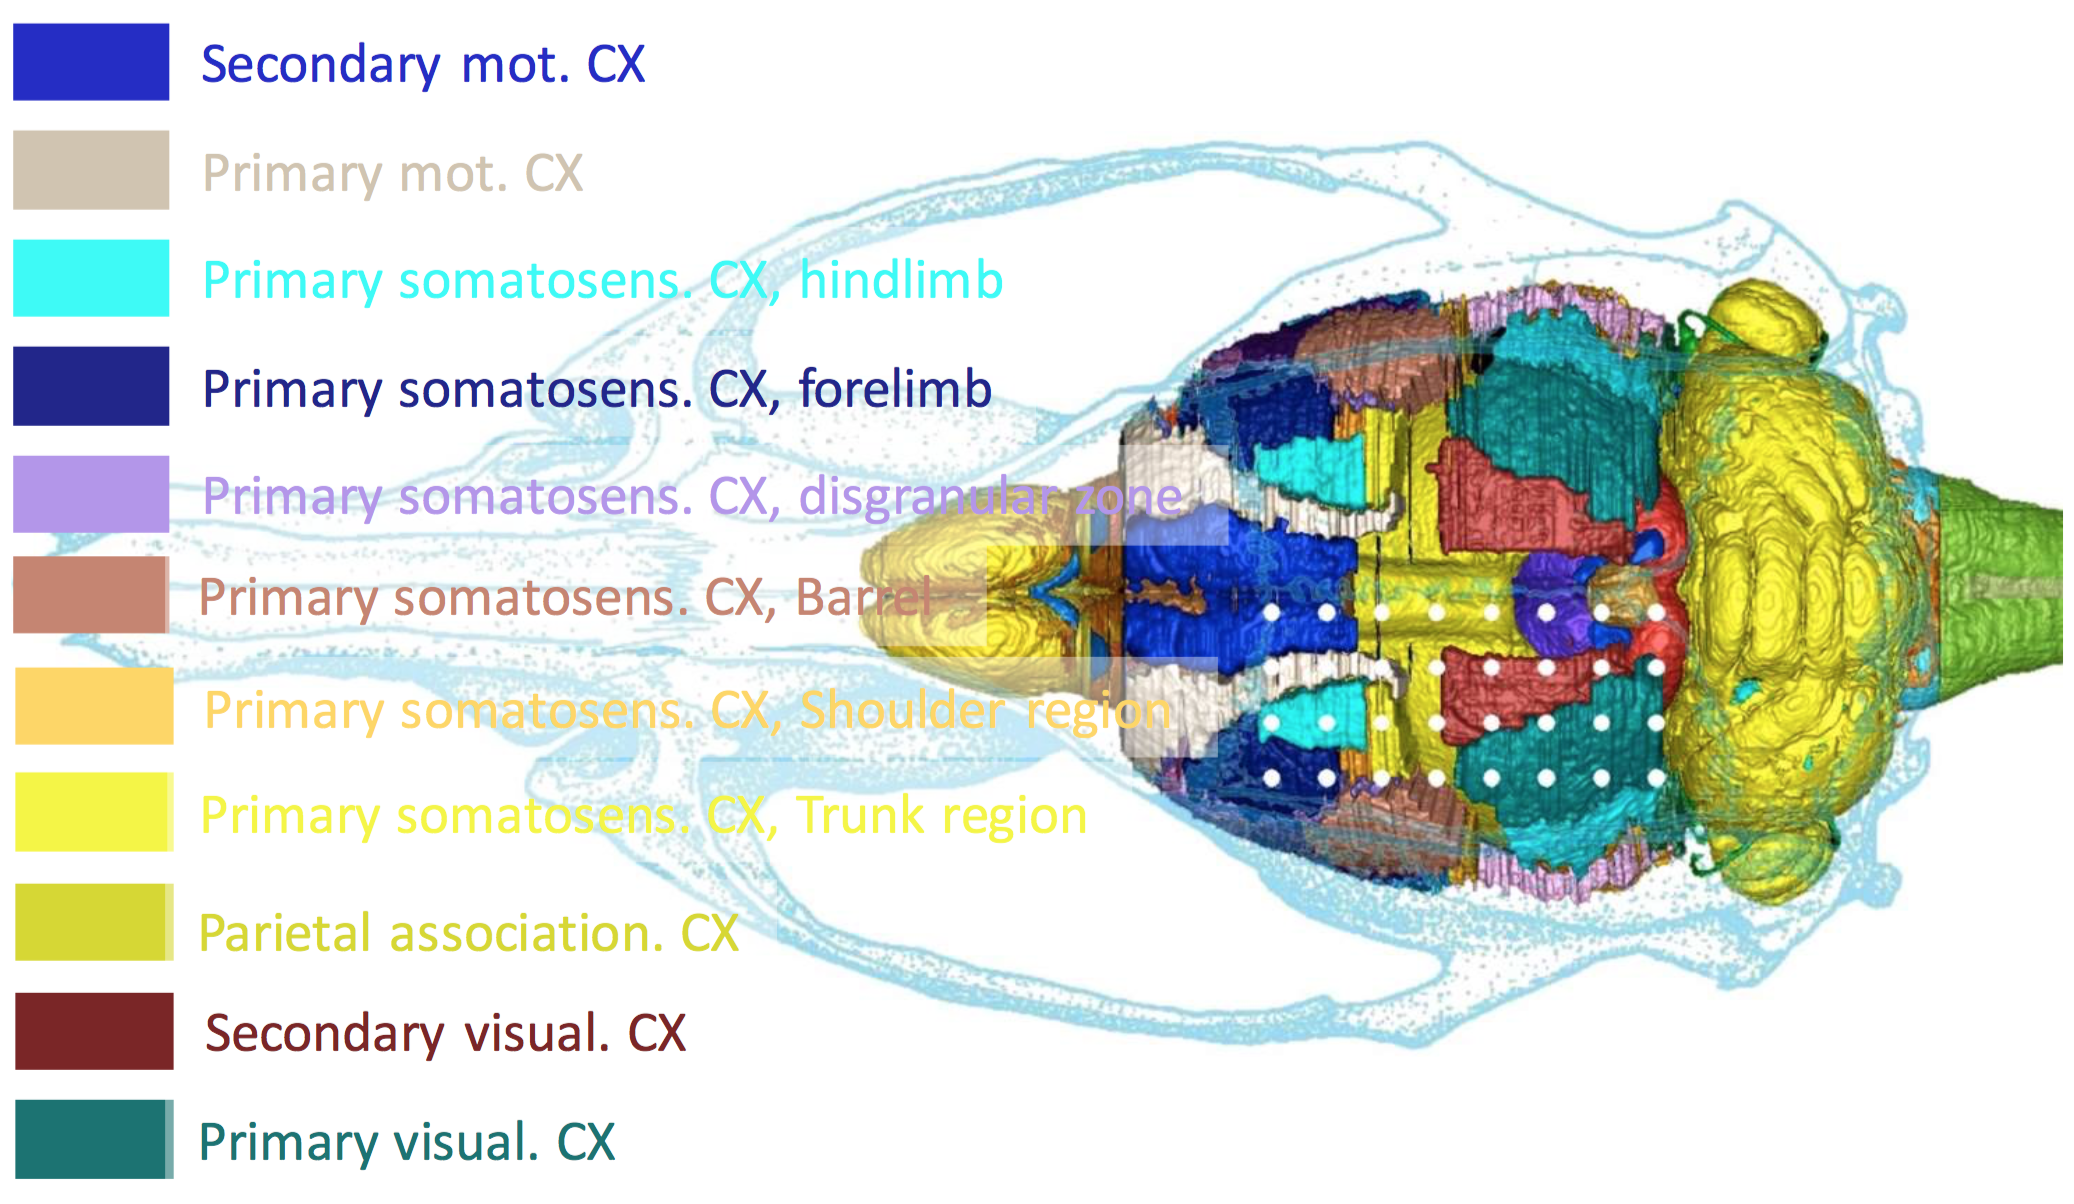
\includegraphics[width=0.95\linewidth]{figures/rat_brain_schematic.png}
    \caption{}
  \end{subfigure}
  \begin{subfigure}[b]{0.45\textwidth}
    \centering
    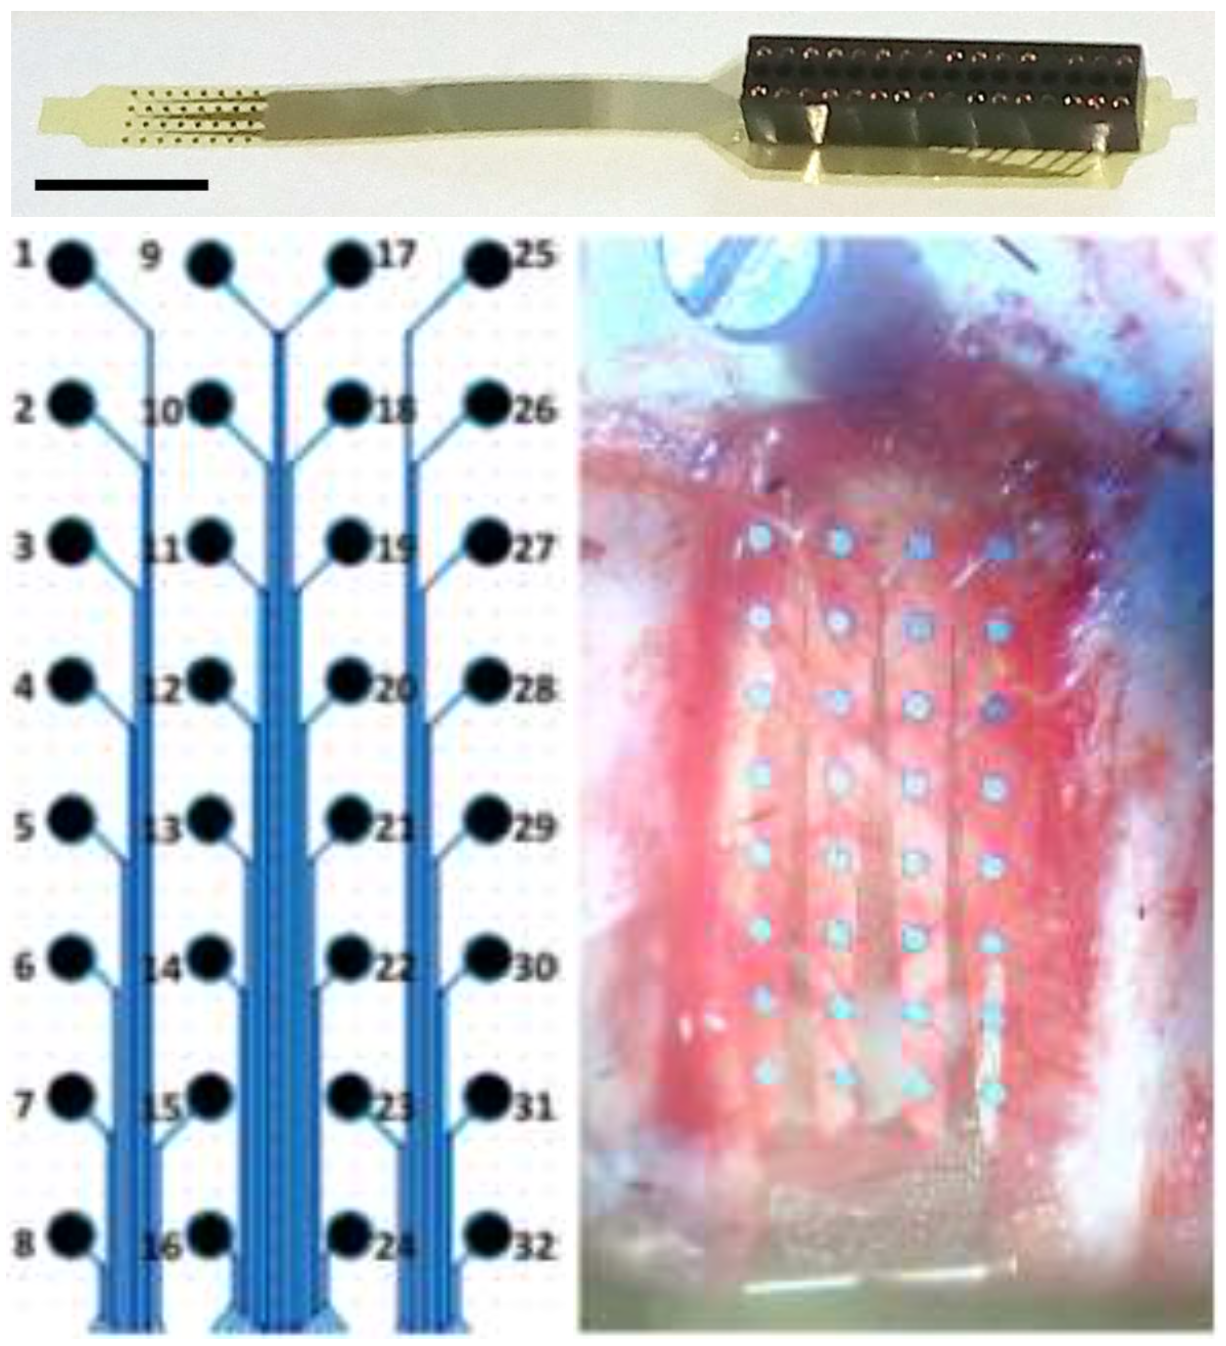
\includegraphics[width=0.95\linewidth]{figures/rat_scull_and_instrument.png}
    \caption{}
  \end{subfigure}
  \caption{(a) A composite drawing showing the brain in the scull. The 3D reconstruction of the brain has been made using the maps of the Paxinos atlas, and the localization of cortical areas are indicated by different colors. White points indicate the position of the recording sites of the membrane electrode. Names for the cortical areas are also shown (based on Hjornevik \textit{et al.} and Paxinos \textit{et al.} \cite{hjornevik2007} \cite{paxinos2009}). (b) Photograph of a membrane electrode shows the construction on the top, the numbering (bottom right) and the surgical implantation (bottom left) is also shown. Electrode 1 malfunctioned during recording.}
  \label{fig:rat_experiment}
\end{figure}


\begin{figure}[H]
  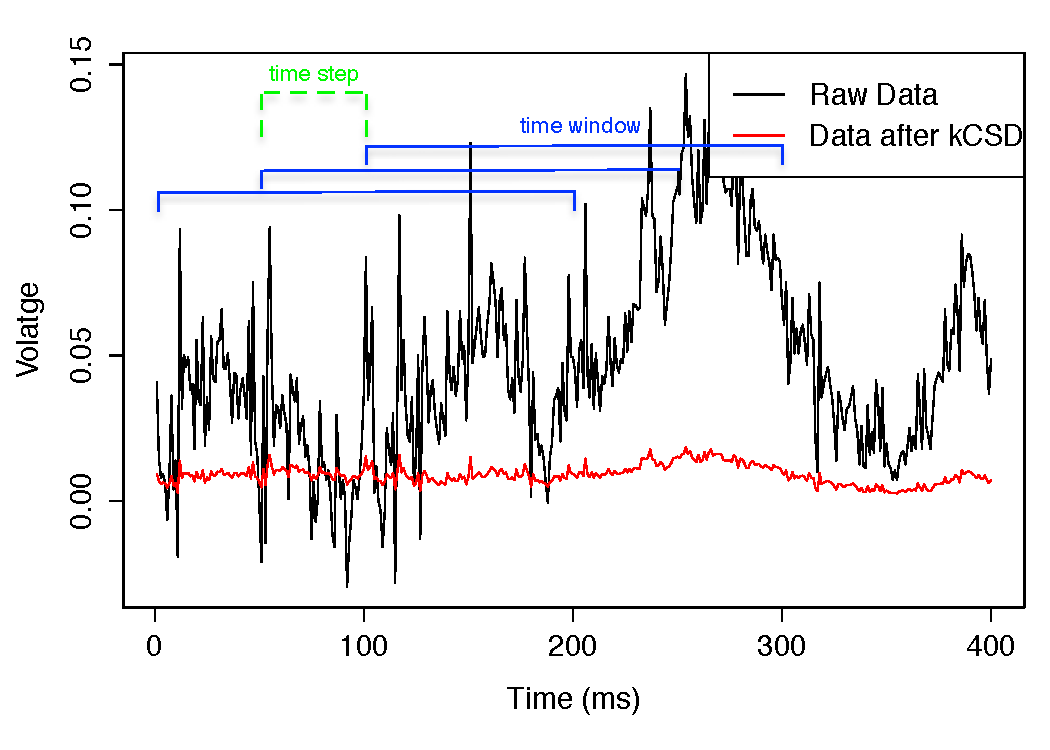
\includegraphics[width=\linewidth]{figures/sample_eeg_signal_with_kcsd_edited.pdf}
  \caption{Sample data from electrode 1, in both its raw form and then in its form after kCSD transformation. Applying kernel Current Source Density extracts the true relationship of neural activity, and in theory eliminates disturbances that might be caused by signal interference. Three sample blue lines are drawn to demonstrate the sliding windows that were used to calculate Sugihara Causality between brain regions. In each time window, the causality was calculated between each brain region, and the time window was moved by an amount \textit{time step}. Different configurations were used for the time window and time step, as reported in table \ref{tab:sliding_window_configuration}. Here, the configuration shown has time window as $200$ and time step as $50$.}
  \label{fig:example_eeg_and_kcsd}
\end{figure}

\begin{table}[H]
\centering
\caption{Configurations used for the sliding window when calculating Sugihara causality that was used as a measure of brain communication. These configurations inform our model of the granularity of brain communication. Since we do not know exactly how quickly information is being passed down from region to region, arbitrary choices were made to test how well each performs and make a more informed decision in future research.}
\label{tab:sliding_window_configuration}
\begin{tabular}{|c|c|c|}
\hline
 Dataset name &  Time window &  Time step \\ \hline
 
 dataset 50 & 200 & 50  \\ \hline
 dataset 200 & 200 & 200 \\ \hline
 dataset 250 & 2000 & 250  \\ \hline
\end{tabular}
\end{table}

\subsubsection{Data Preprocessing}
Kernel Current Source Density (kCSD) method was used on the grid of channels to account for possible electrical interference with the direct measurement (Fig. \ref{fig:example_eeg_and_kcsd}) \cite{Potworowski2012}. The measured potentials produced by kCSD arise as the linear combination of the trans-membrane currents, which is a more direct and localized quantity to measure the neural activity. Therefore current source density distribution was calculated by the kCSD method and used for the analysis instead of the original EEG signals.

Afterwards, in order to reduce the data size that is operated on, we lumped channels from the same brain regions together by averaging them (Fig. \ref{fig:brain_region_lumping}). In addition to reducing dimensionality, this process also puts emphasis of causality on functional brain regions instead of a local cluster of neurons. 

\subsubsection{Sugihara Causality Measurement}
After lumping the kCSD signals from the same region, we perform Sugihara Causality calculation on the regions by using a sliding windows method (Fig. \ref{fig:example_eeg_and_kcsd}). Because we do not know how granular of a time frame the brain uses to communicate (and how that affects the EEG signal we record), we use three different time scales as reported in table \ref{tab:sliding_window_configuration}. This produces 3 datasets with similar characteristics. The important thing to keep in mind is that after this step, each causality measure that resulted from the Sugihara Causality analysis is a measure of how much one region is affecting the other, and we use that as a way to describe brain communication and information flow. Each causality measure is therefore an \textit{edge} of communication from one region to another, meaning that each brain region is a node and each causality measure is a weighted edge. Figure \ref{fig:sample_graph} shows a sample graph constructed from joining all the causality measures from a specific time window. This is essentially a (theoretical) snapshot of how each brain region was affecting other brain regions in that time window.

\begin{figure}[H]
  \centering
  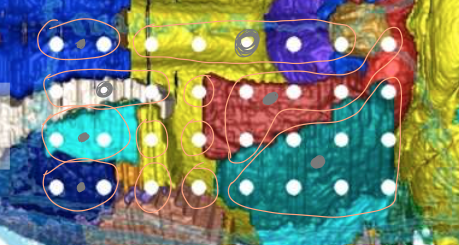
\includegraphics[width=0.65\linewidth]{figures/brain_region_lump.png}
  \caption{The distribution and lumping of the brain regions in the brain. A total of 12 region channels were constructed from the initial 31 local channels. The schematic is based on rat brain atlas mapping.}
  \label{fig:brain_region_lumping}
\end{figure}


\begin{figure}[H]
  \centering
  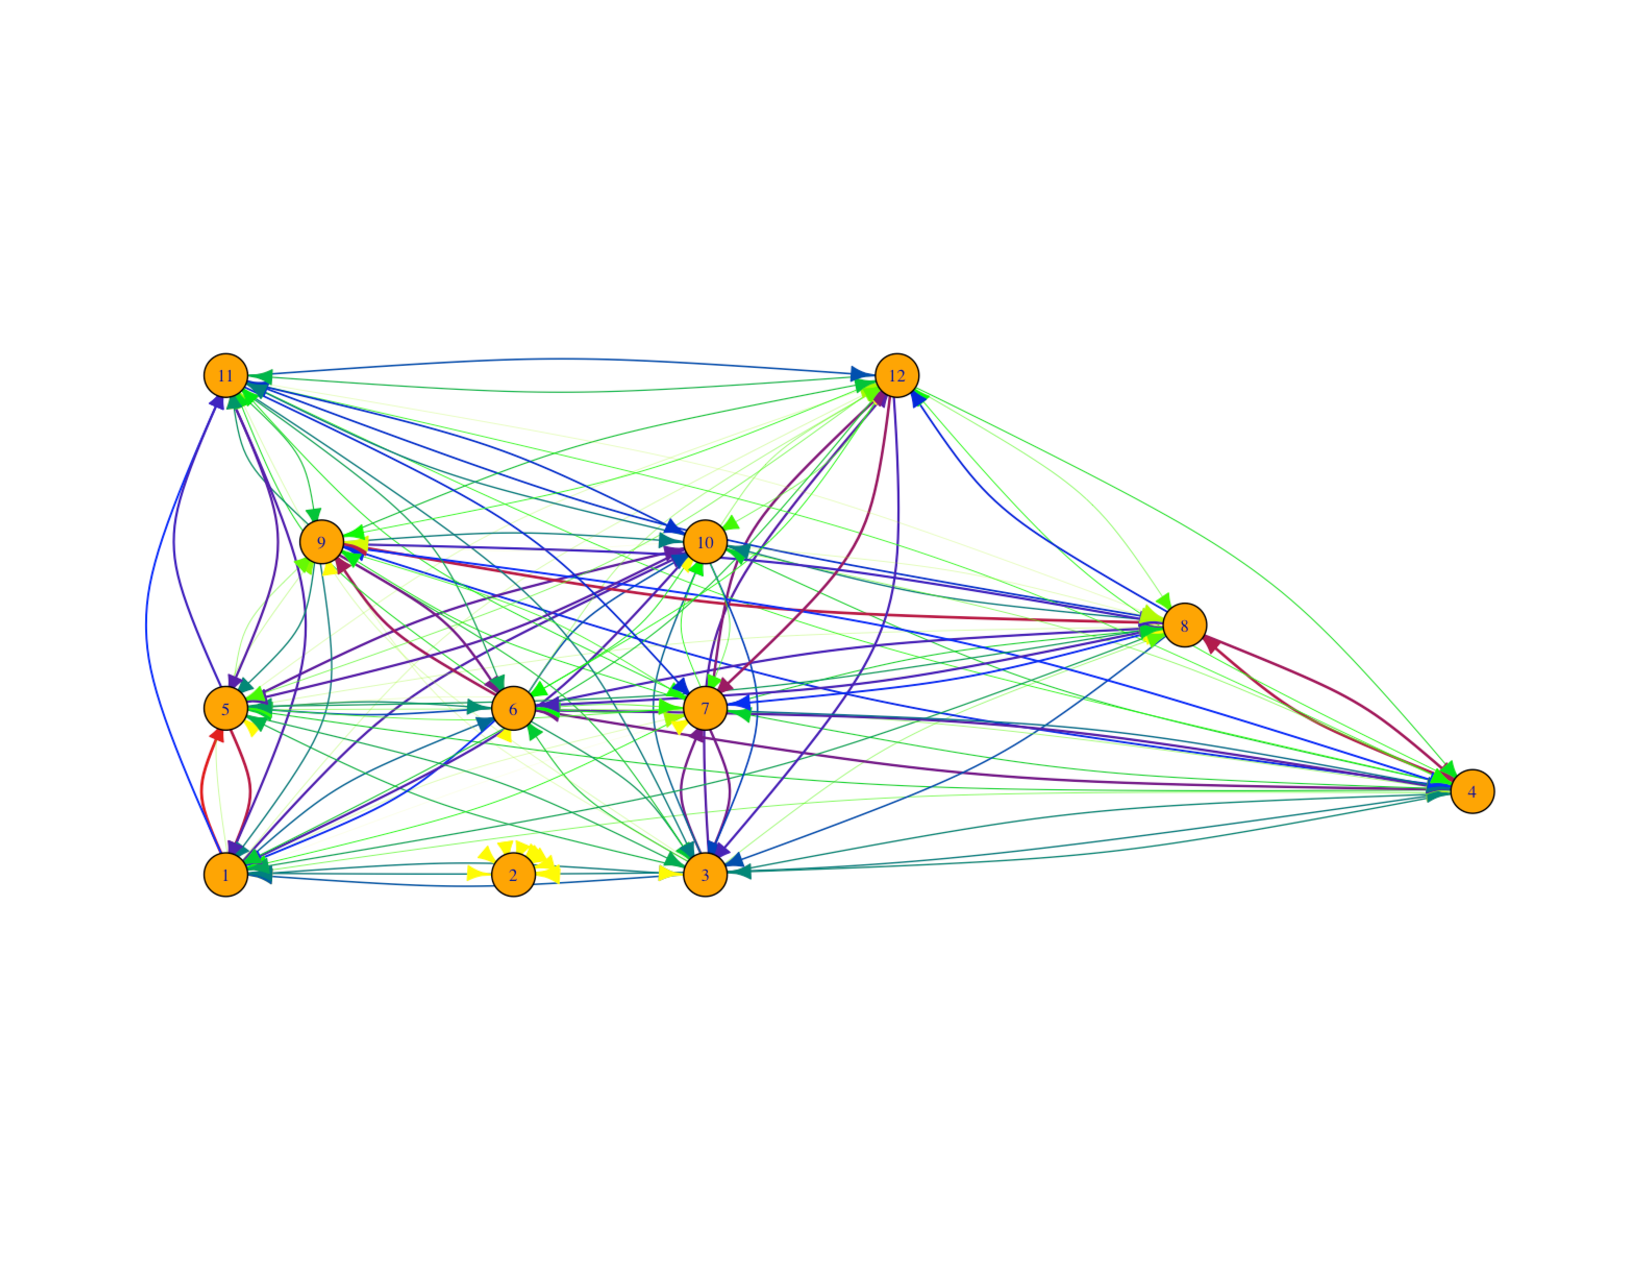
\includegraphics[width=0.55\linewidth]{figures/sample_graph.pdf}
  \caption{Sample graph constructed from calculating the Sugihara causality between brain regions. Lumped brain regions correspond to the gray circular mapping in Fig. \ref{fig:brain_region_lumping}. Edge colors represent the strength of the causal relationship. From weakest to strongest: Yellow, Green, Blue, Red. The edge weight ranges from 0 to 1.}
  \label{fig:sample_graph}
\end{figure}


\subsection{Problem Statement}

Given a mesh of EEG signals that have been translated into a brain region communication graph series, can we cluster the graphs into meaningful segments that can help us find epilepsy states. To find out, we plan to use unsupervised clustering in the form of Gaussian Mixture algorithm. We also employ principal component analysis (PCA) to help reduce the dimensionality of the data for faster processing time.

% In this section, you will need to clearly define the metrics or calculations you will use to measure performance of a model or result in your project. These calculations and metrics should be justified based on the characteristics of the problem and problem domain. Questions to ask yourself when writing this section:

% Are the metrics you’ve chosen to measure the performance of your models clearly discussed and defined?
% Have you provided reasonable justification for the metrics chosen based on the problem and solution?
\subsection{Metrics}
The unsupervised learning used here along with the high dimensionality of the dataset used in this project bring with them a unique difficulty in terms of defining a clear scoring method. In the scikit-learn library, there are only two methods that can be used to give a score to clusters (assuming no knowledge of \textit{true} labels of each data point): Silhouette Coefficient and Calinsky-Harabaz Index. Both scores ascertain the quality of clustering by measuring how dense, well defined, and separated the clusters are. We are forced to use these metrics due to the nature of the data we are given, as we don't know the true labels of the data points. However, we do know the specific times of when epilepsy was induced, and since epilepsy is \textit{one} state in the brain, then we can use the time indecies for epilepsy to be the one cluster we perform an accuracy (possibly F1) metric on.

\section{Analysis}
% (approx. 2-4 pages)

\subsection{Data Exploration and Visualization}
The data we produced is a series of complete, directed graphs (all the same topology; each node is a brain region as seen in figure \ref{fig:rat_experiment}; each edge is a causality/communication measure) and their edge weights that we refer to as $\rho$ scores. For each graph, there are $132$ $\rho$ scores, all of which range between 0 and 1 (decimals). Most of the $\rho$ scores appear to be of high values, suggesting high connectivity between brain regions and therefore a high density graph (Fig. \ref{fig:rho_hist_all_experiment}). Furthermore, we also notice that many of the $\rho$ scores to be similar within a pair of nodes (Fig. \ref{fig:diff_within_pair_hist}). For example, when looking at regions 1 and 2 within the first 200 milliseconds, they appear to be equally communicating to one another (Fig. \ref{fig:sample_pair_causality_plot}). This could be indicative of either bidirectional causality or unidirectional forcing, both of which can be detected by the Sugihara model.


\begin{figure}[H]  
	\centering
	\begin{subfigure}{0.45\textwidth}
		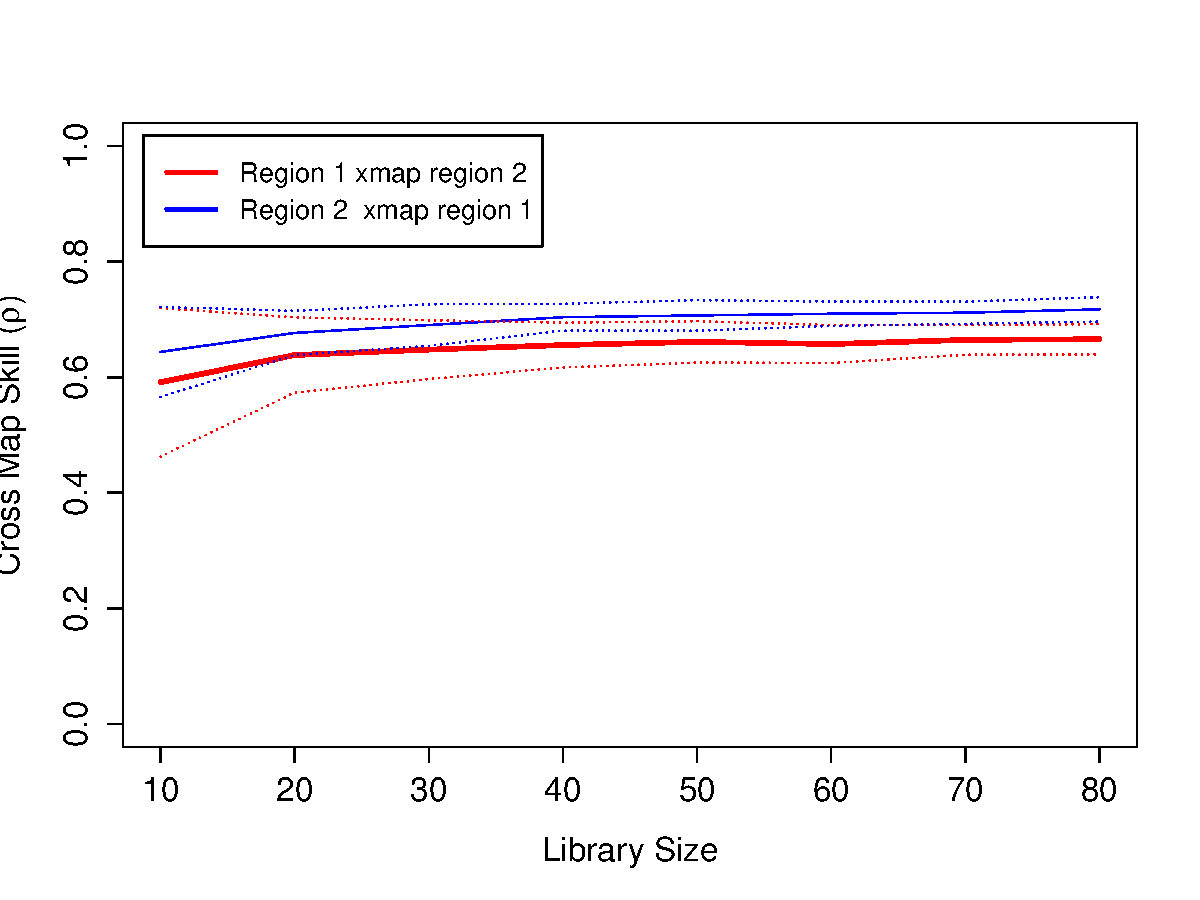
\includegraphics[width=\linewidth]{figures/sample_pairwise_causality_measure.pdf}
		\caption{}
		\label{fig:sample_pair_causality_plot}
	\end{subfigure}
	\begin{subfigure}{0.45\textwidth}
		\centering
		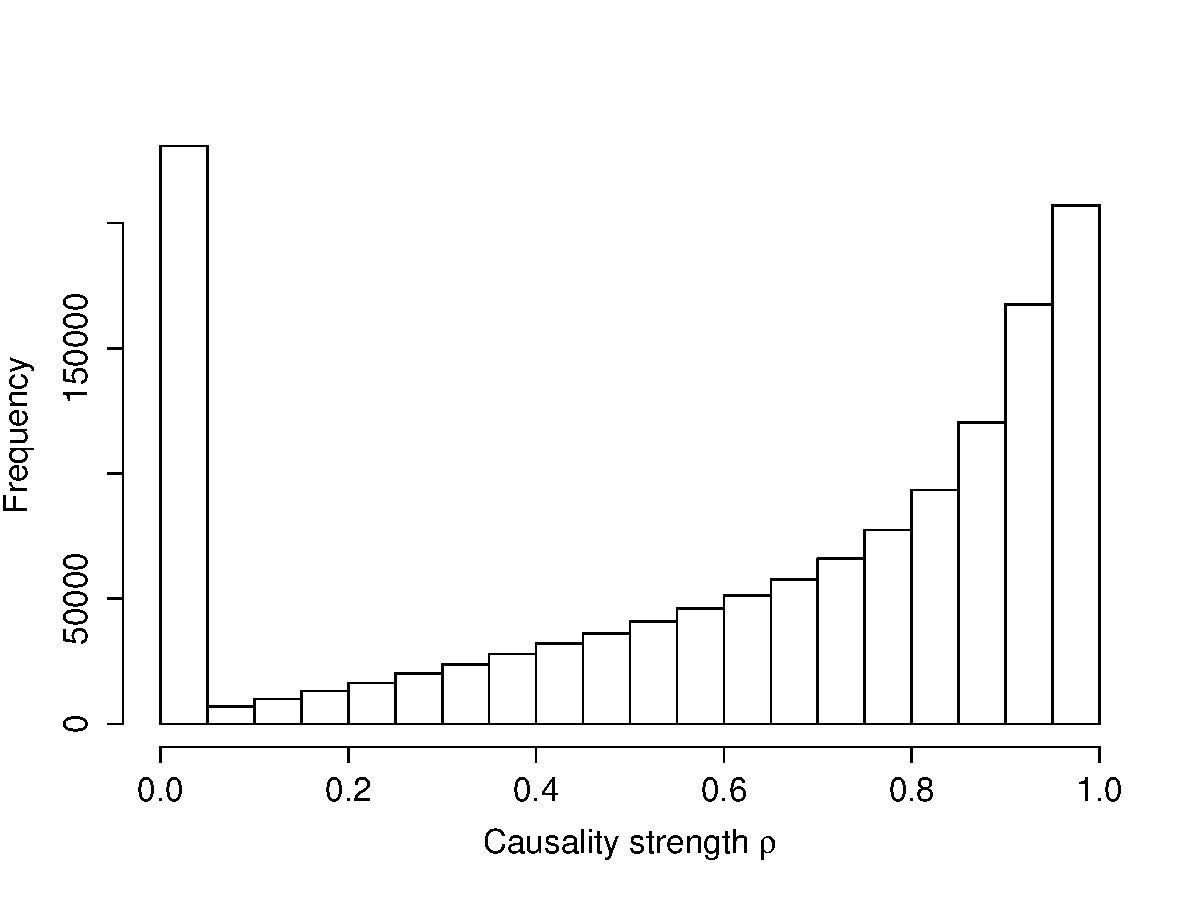
\includegraphics[width=1\linewidth]{figures/rho_hist_all_experiment.pdf}
		\caption{}
		\label{fig:rho_hist_all_experiment}
	\end{subfigure}
	\caption{(a) A sample graph plotting the convergent cross mapping skill ($\rho$) between region (nodes) 1 and 2 during the first 200 ms of the experiment. The skill mapping channel 1 to channel 2 is very similar to the one mapping channel 2 to channel 1. This might infer either bidirectional causality or unidirectional forcing. A similar pattern (close $\rho$ value between pairs) was found for most of the pairs of edges. (b) The distribution of CCM skill ($\rho$) during the entire experiment. Many relationships appear to be causal in the brain, with equally as many being non-causal throughout the experiment. Causality was calculated from signals of lumped regions after calculating the CSD. Cross mapping was done on every pair of regions with library size of 80, and each pair has two causality directions. Sliding windows of 200 ms were used, with a sliding step of 50 ms.}
\end{figure}

\begin{figure}[H]
  \begin{subfigure}{.48\textwidth}
    \centering
    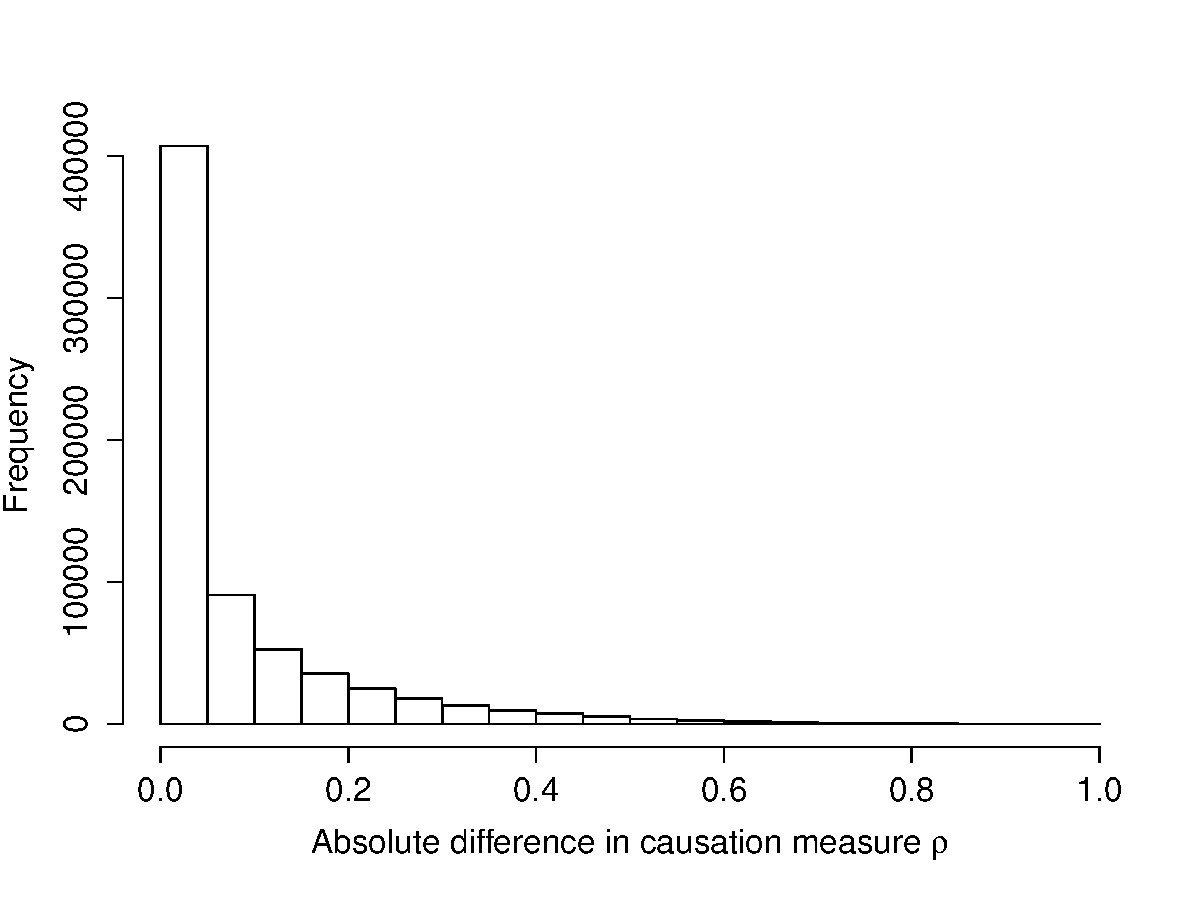
\includegraphics[width=0.95\linewidth]{figures/diff_within_pair_hist.pdf}
    \caption{Absolute difference of $\rho$ between all pairs}
  \end{subfigure}  
  \begin{subfigure}{.48\textwidth}
    \centering
    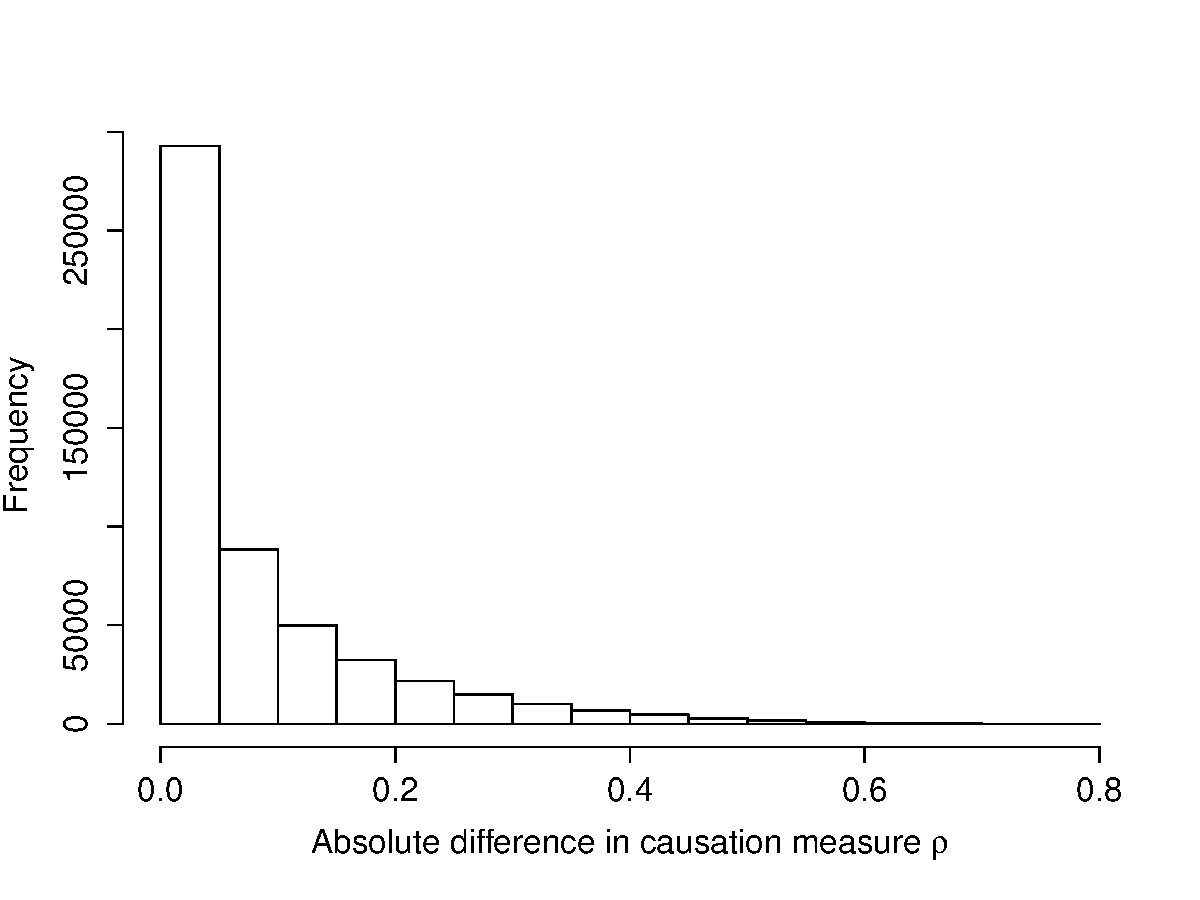
\includegraphics[width=0.95\linewidth]{figures/diff_within_pair_over_2_hist.pdf}
    \caption{Absolute difference of $\rho$ between pair both of which is at least 0.2}
  \end{subfigure}
  \caption{Difference of causality values within a pair is small, even when accounting for non-existing relationships where both causalities are below 0.2. This similarity between directions of causality in a pair could imply a bidirectional relationship between most regions, or could alternatively imply a unidirectional forcing (synchrony) phenomenon. Sliding windows of 200 ms were used, with a sliding step of 50 ms. A library size of 80 was used.}
  \label{fig:diff_within_pair_hist}
\end{figure} 

% In this section, you will be expected to analyze the data you are using for the problem. This data can either be in the form of a dataset (or datasets), input data (or input files), or even an environment. The type of data should be thoroughly described and, if possible, have basic statistics and information presented (such as discussion of input features or defining characteristics about the input or environment). Any abnormalities or interesting qualities about the data that may need to be addressed have been identified (such as features that need to be transformed or the possibility of outliers). Questions to ask yourself when writing this section:

% If a dataset is present for this problem, have you thoroughly discussed certain features about the dataset? Has a data sample been provided to the reader?
% If a dataset is present for this problem, are statistics about the dataset calculated and reported? Have any relevant results from this calculation been discussed?
% If a dataset is not present for this problem, has discussion been made about the input space or input data for your problem?
% Are there any abnormalities or characteristics about the input space or dataset that need to be addressed? (categorical variables, missing values, outliers, etc.)
%
% In this section, you will need to provide some form of visualization that summarizes or extracts a relevant characteristic or feature about the data. The visualization should adequately support the data being used. Discuss why this visualization was chosen and how it is relevant. Questions to ask yourself when writing this section:

% Have you visualized a relevant characteristic or feature about the dataset or input data?
% Is the visualization thoroughly analyzed and discussed?
% If a plot is provided, are the axes, title, and datum clearly defined?

\subsection{Algorithms and Techniques}
For the clustering, we choose the Gaussian Mixture algorithm as implemented by the Sci-kit learn python library. Gaussian Mixture Model (GMM) clustering can be thought of as a K-means algorithm that is generalized to account for the covariance of the data and centers of the Gaussian distributions. Because of this feature, while K-means algorithm only clusters data points in spherical shapes, the GMM model allows clusters to take many shapes. For these reasons, the GMM would be a more suitable algorithm to use in our case. GMM has a few parameters that could be tuned, the most important of which is the covariance type (full, tied, diagonal, or spherical) which dictates how the cluster edges are expanded and how the clusters grow. This parameter will be fine tuned using grid search. 
% In this section, you will need to discuss the algorithms and techniques you intend to use for solving the problem. You should justify the use of each one based on the characteristics of the problem and the problem domain. Questions to ask yourself when writing this section:

% Are the algorithms you will use, including any default variables/parameters in the project clearly defined?
% Are the techniques to be used thoroughly discussed and justified?
% Is it made clear how the input data or datasets will be handled by the algorithms and techniques chosen?
\subsection{Benchmark}
Since this method has never been attempted before (using Sugihara Causality graphs to identify epilepsy), providing a succinct and complete benchmark is a difficult task. Furthermore, the clustering here is used to explore whether or not there are any extractable information from causal networks in the brain, and whether the brain communicates differently when it is suffering from epilepsy compared to when it is operating normally. 

Keeping this in mind, we rely on the simple F1 score to provide a simple reliability measure of how well the clustering is separating and predicting the epilepsy cluster. Since we know that epilepsy doesn't happen often in our dataset (only ~20 seconds  of epilepsy related events in our ~500 seconds dataset), we can assign the cluster with the least data points as the epilepsy one, and then measure how exclusive the epilepsy cluster is to the times when epilepsy was \textit{actually} happening by measuring an F1 score. Since our epilepsy happens for about 4\% of the dataset, then the baseline score we expect should be 96\% of accuracy and 0.99 F1 score. These scores are attained if all the data points were labeled as one (non-epilepsy) cluster.

% In this section, you will need to provide a clearly defined benchmark result or threshold for comparing across performances obtained by your solution. The reasoning behind the benchmark (in the case where it is not an established result) should be discussed. Questions to ask yourself when writing this section:

% Has some result or value been provided that acts as a benchmark for measuring performance?
% Is it clear how this result or value was obtained (whether by data or by hypothesis)?
\section{Methodology}

% (approx. 3-5 pages)

\subsection{Data Preprocessing}

Some of our edge weights had some Not A Numerical values, and those were altered to 0, which is the lowest $\rho$ score possible. Once that error was corrected and the data has been put in the graph series format, separated into the three different datasets, we perform Principal Component Analysis (PCA) to reduce the dimensionality of the datasets. This both gives us insight into what components of the graph are logically important for the model and helps decrease the time required to run our model. The results of PCA was used to create three different datasets from each dataset: a dataset that covered 80\% of the variance, a dataset that covered 90\% of the variance, and a dataset that covered 99\% of the variance. This was done to test how dimensionality reduction would affect the final clustering efforts. If the scoring for the reduced datasets with only 80\% of the variance is similar to the scoring of the reduced datasets with 99\% of the variance, then we use the less dimensional reduced datasets even though they give us a less accurate version of the original information. A list of the PCA datasets and their different variance levels are reported in table \ref{tab:pca_datasets}. After the principal component analysis was done on the datasets, the components required to reach the threshold levels of 80, 90, and 99 percents were recorded in table \ref{tab:components_needed_for_variance} (Fig. \ref{fig:pca_analysis_variance}).


\begin{table}[H]
\centering
\caption{Dataset names for the result of PCA analysis. Three different reduced datasets are produced each of which keeps a certain percentage of the original variance. Since we started with three datasets and created three new ones out of each by applying PCA with different levels of components, we arrive at 9 total reduced datasets.}
\label{tab:pca_datasets}
\begin{tabular}{|c|c|c|c|}
\hline
  &  80\% variance &  90\% variance & 99\% variance \\ \hline
 
dataset 50 & reduced 50 80 & reduced 50 90 & reduced 50 99  \\ \hline
dataset 200 & reduced 200 80 & reduced 200 90 & reduced 200 99  \\ \hline
dataset 250 & reduced 250 80 & reduced 250 90 & reduced 250 99  \\ \hline
\end{tabular}
\end{table}


\begin{figure}[H]
  \centering
  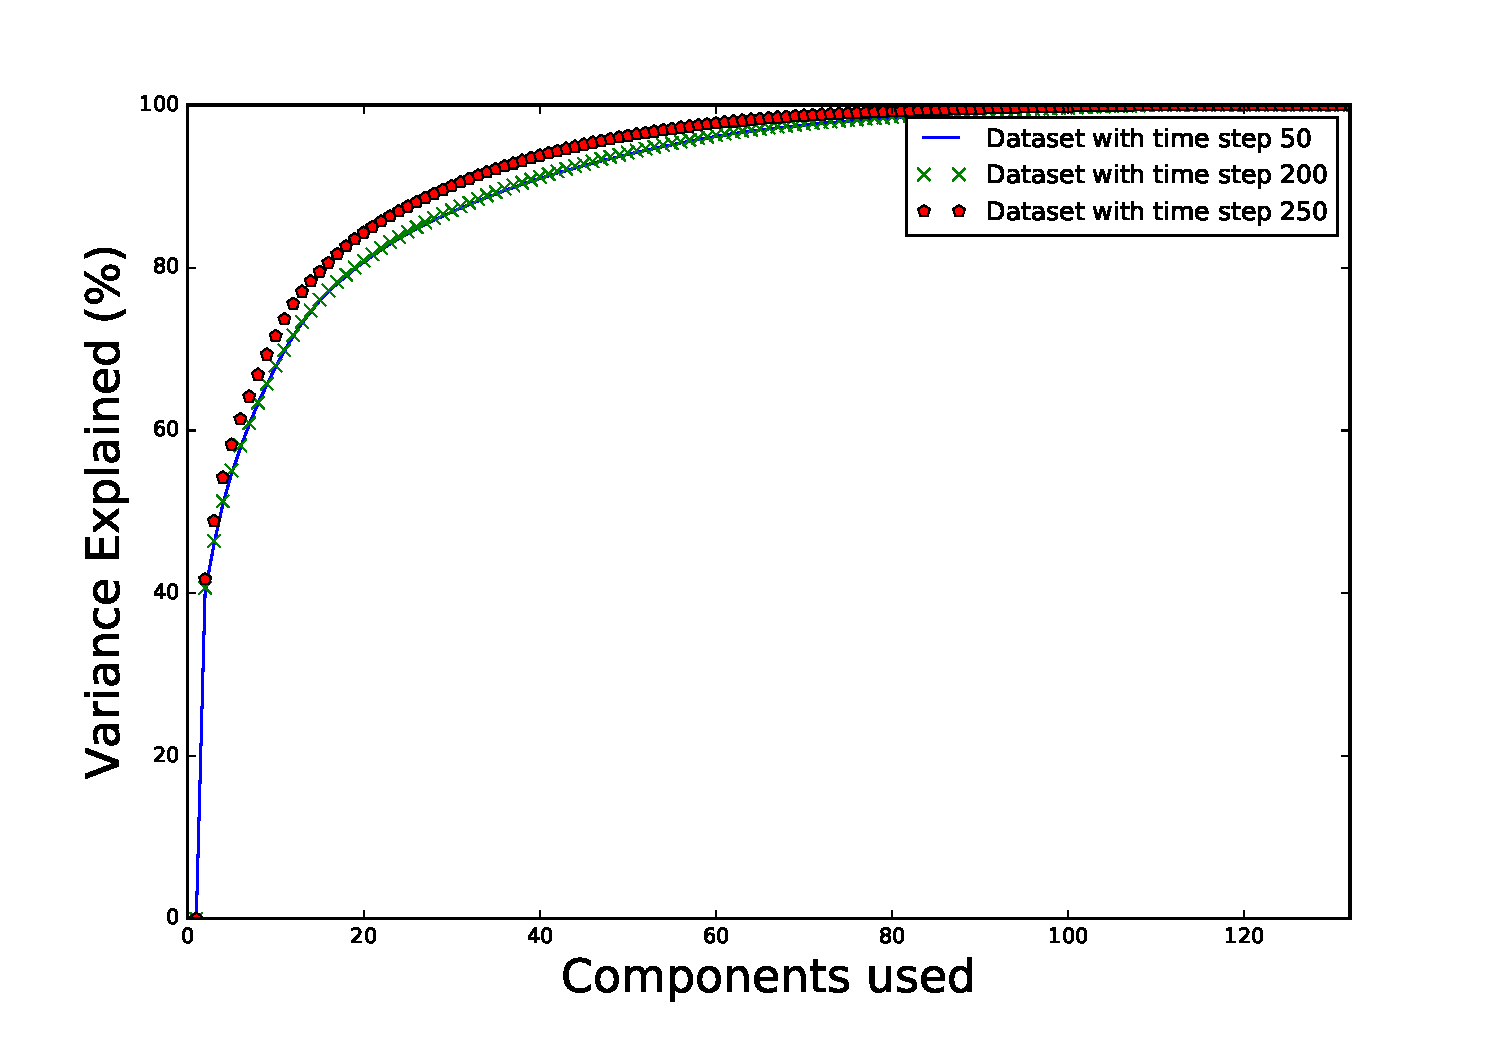
\includegraphics[width=0.55\linewidth]{figures/variance_explained_with_pca.pdf}
  \caption{Principle Component Analysis conducted on the three datasets reveals that the overall variance of the data can be maintained by using only a subset of the edges of the graph rather than all of them. The dataset with a time step of 250 ms needs less components to explain the variance than the other two, while the datasets with 200 and 50 ms time steps showed an almost exact level of variance explained with the number of components. This suggests that the 250 ms dataset is not complex enough, which might indicate that 2000 ms is too big of a time frame to record the granular communication speed of the brain.}
  \label{fig:pca_analysis_variance}
\end{figure}

\begin{table}[H]
\centering
\caption{Different component numbers are needed for each dataset to maintain a certain level of variance explained using PCA for dimensionality reduction. These values for components required for reaching a score standard were used to produce reduced forms of the datasets as noted in table \ref{tab:pca_datasets}. These reduced forms of the datasets were then analyzed in figure \ref{fig:silhouette_scores}.}
\label{tab:components_needed_for_variance}
\begin{tabular}{|c|c|c|c|}
\hline
 &  80\% variance explained &  90\% variance explained & 99\% variance explained \\ \hline
 
 Components in dataset 50 & 20 &  38&  87  \\ \hline
 Components in dataset 200 & 20 &  37&  87\\ \hline
 Components in dataset 250 & 16 &  30&  76  \\ \hline
\end{tabular}
\end{table}



% In this section, all of your preprocessing steps will need to be clearly documented, if any were necessary. From the previous section, any of the abnormalities or characteristics that you identified about the dataset will be addressed and corrected here. Questions to ask yourself when writing this section:

% If the algorithms chosen require preprocessing steps like feature selection or feature transformations, have they been properly documented?
% Based on the Data Exploration section, if there were abnormalities or characteristics that needed to be addressed, have they been properly corrected?
% If no preprocessing is needed, has it been made clear why?

\subsection{Implementation}
Once the dimensionality of the data was reduced with PCA, a Gaussian Mixture clusterer was initiated for each dataset from table \ref{tab:pca_datasets}, and all number of clusters from $2$ to $40$ were tried and tested by the Silhouette Coefficient and Calinsky-Harabaz Index scorers (Figs. \ref{fig:silhouette_scores}, \ref{fig:calinsky_scores}).


\begin{figure}[H]
  \centering
  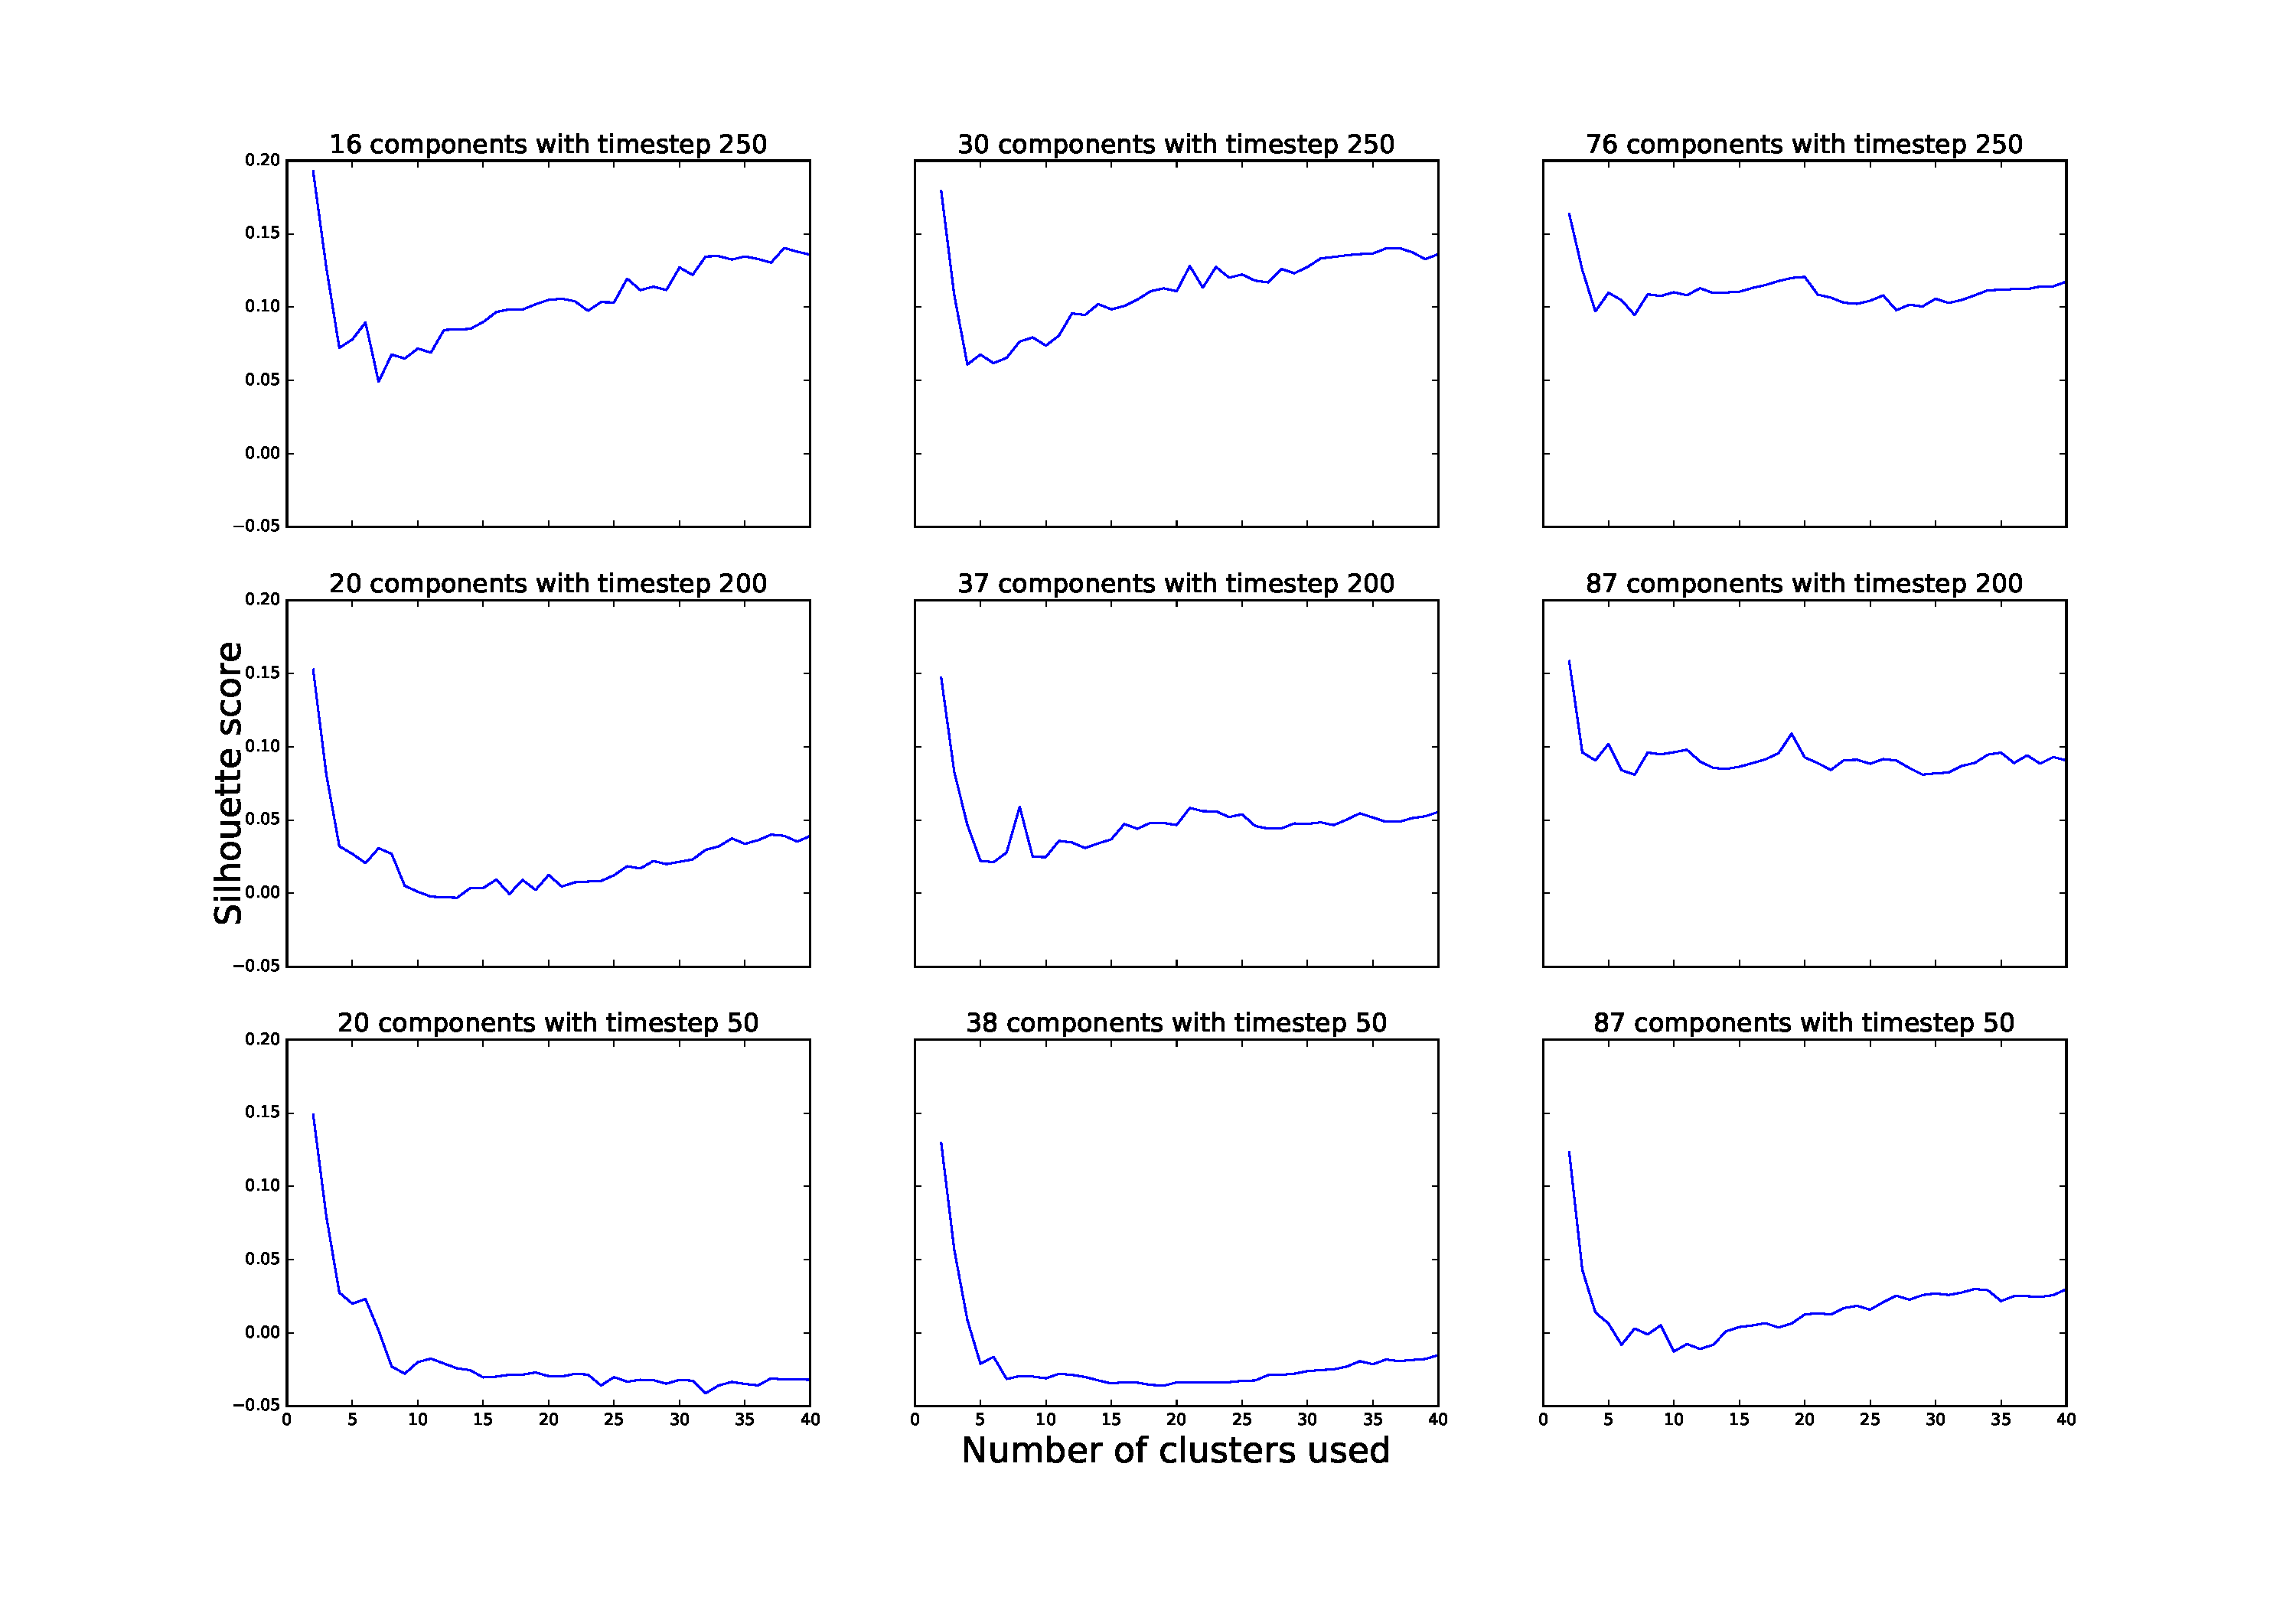
\includegraphics[width=\linewidth]{figures/silhouette_scores.pdf}
  \caption{Silhouette scores for clustering with different cluster numbers. Scores close to 1 suggest clusters that are dense and well separated; scores close to -1 suggest clusters that overlap and are not dense. The best score is consistently when there are only two clusters, and dips greatly when creating more clusters but begins to rise after ~30 clusters. With the dataset 250 and dataset 50, PCA with less components (16 and 20 components respectively) showed a better silhouette score than the other, higher component reduced datasets. However, dataset 200 showed a better silhouette score when more components were used. Especially with a rather thin margin of difference in scores between components, it is difficult to conclude whether having more PCA reductionist approach is beneficial.}
  \label{fig:silhouette_scores}
\end{figure}



\begin{figure}[H]
  \centering
  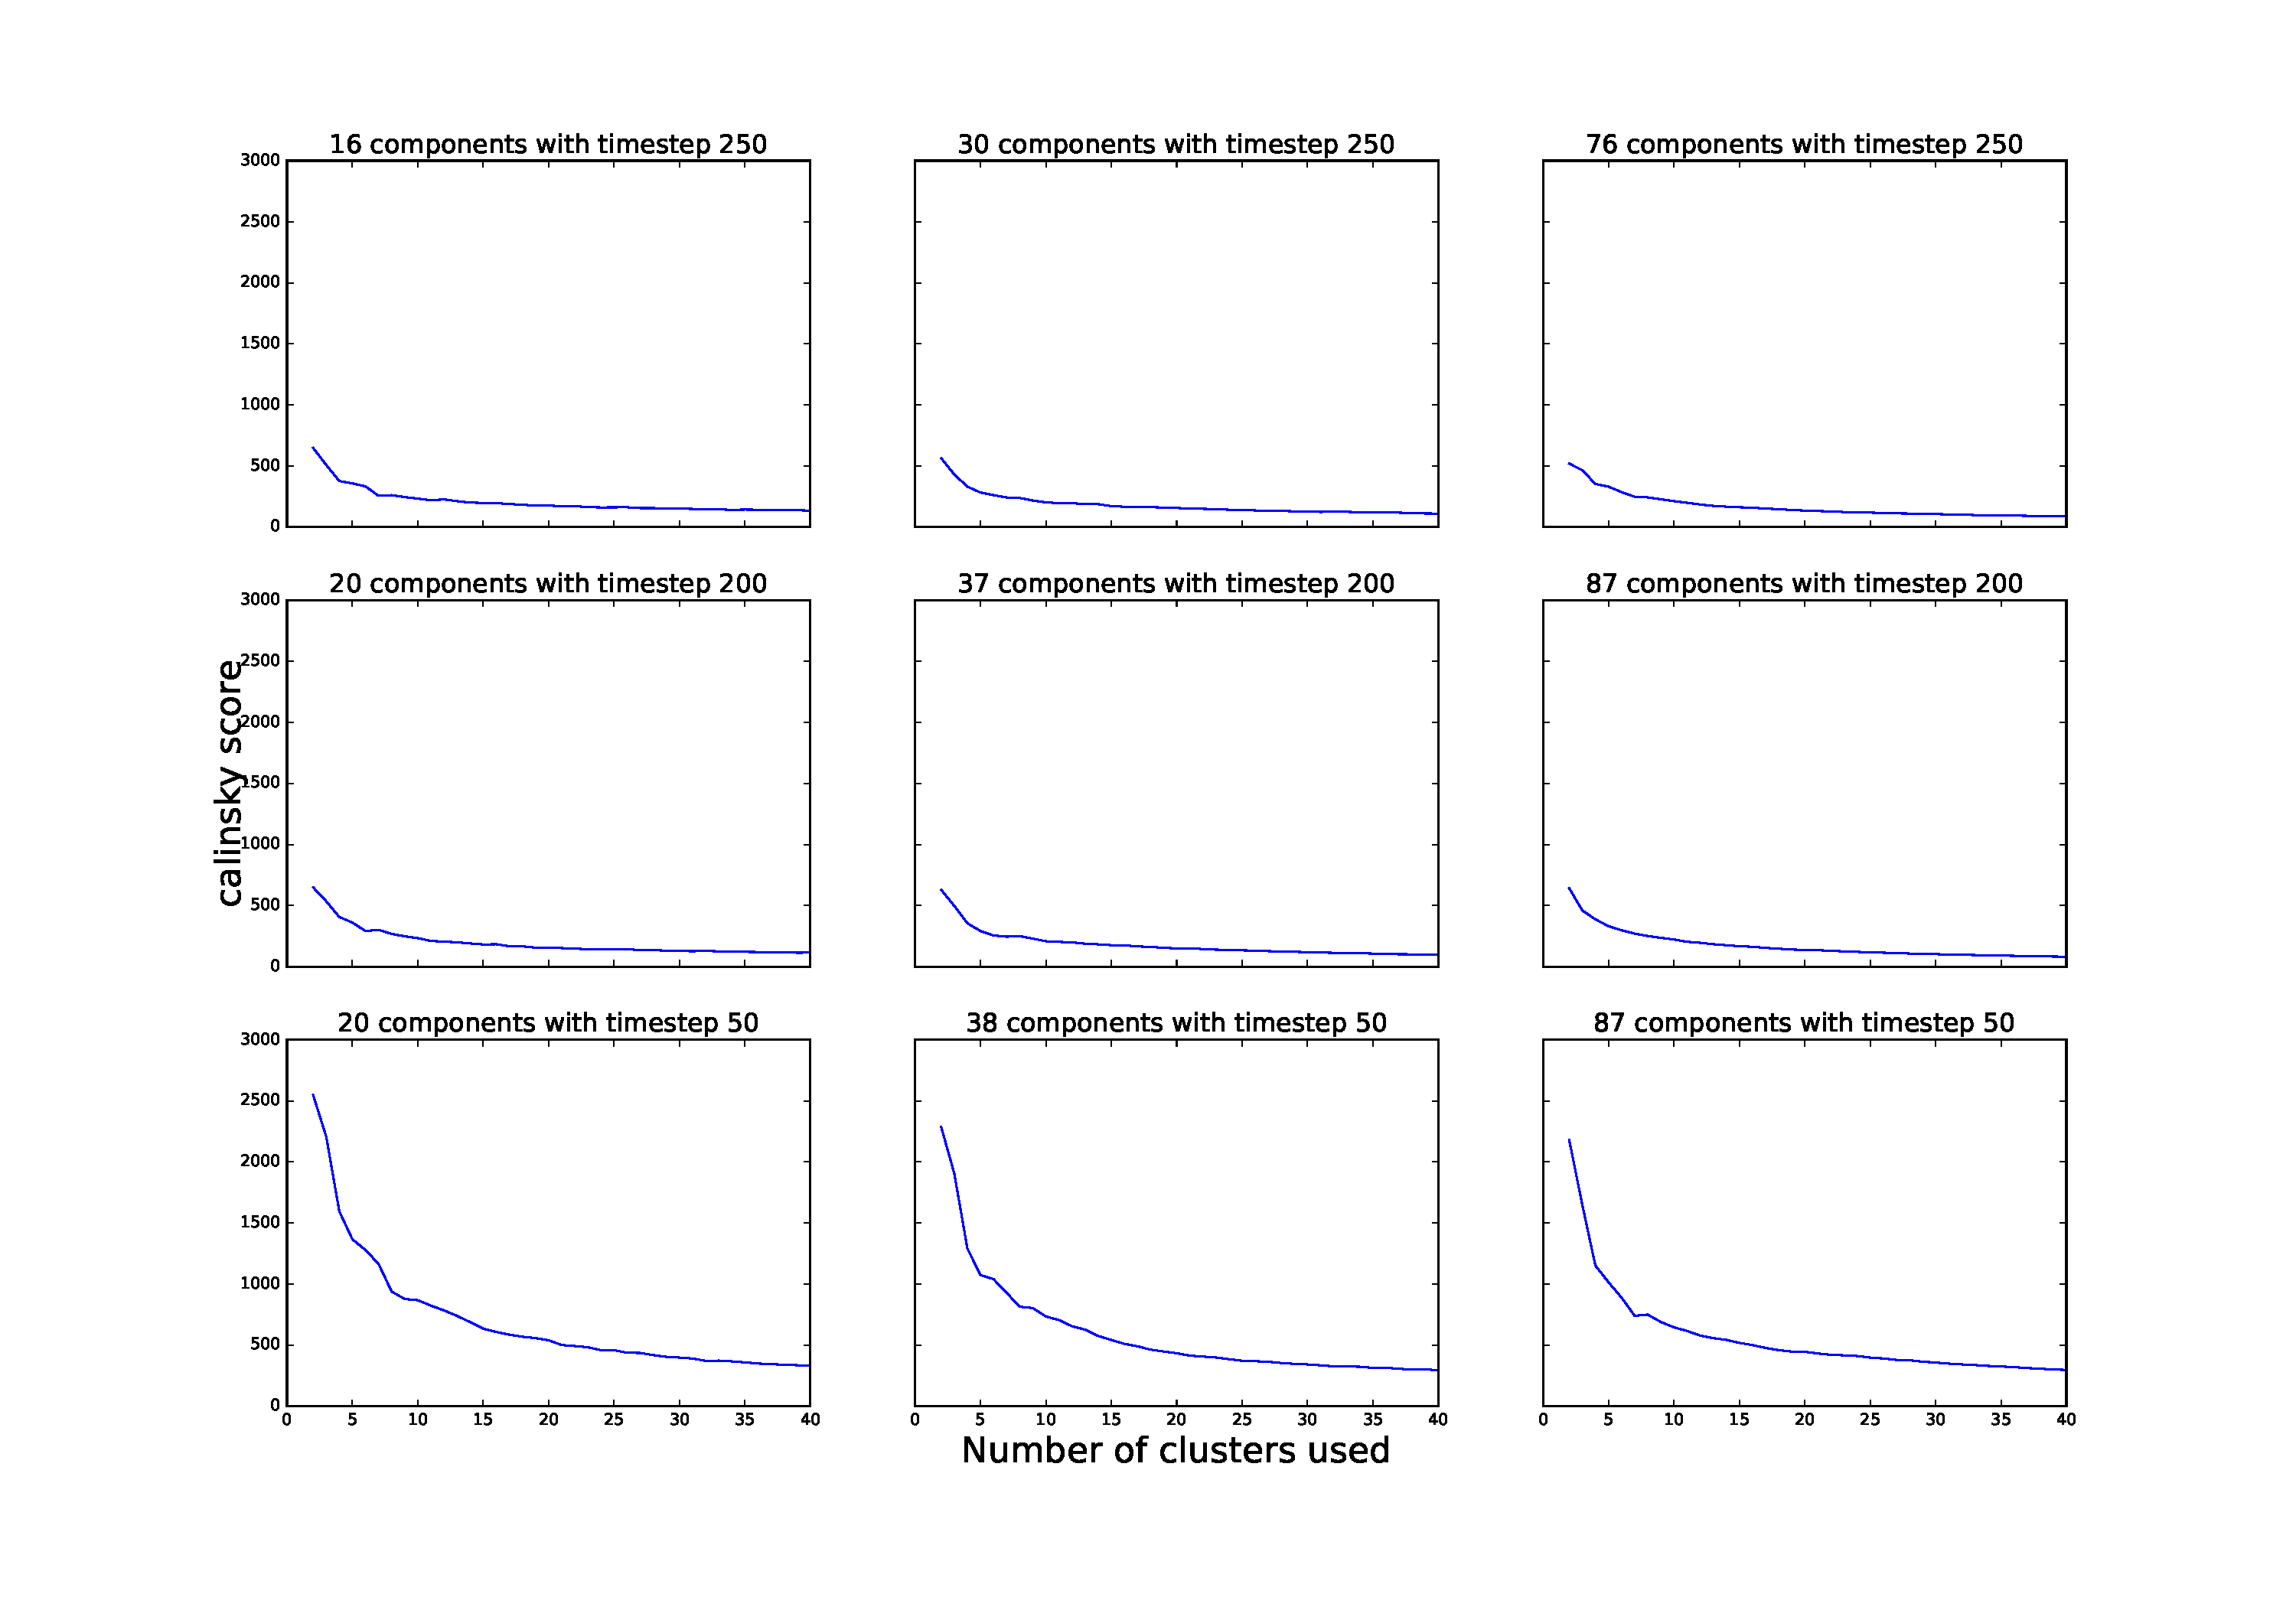
\includegraphics[width=\linewidth]{figures/calinsky_scores.pdf}
  \caption{Calinsky-Harabaz scores for clustering with different cluster numbers. Higher scores mean more separated and dense clusters, which is positive. The score dips greatly when creating more than two clusters, but begins to rise after ~30 clusters. The silhouette scores show that having more components when reducing with PCA results in better clustering scores. The scores also show that scores for the reduced data that keep 99\% of the variance (right column) are all similar in score and trend.}
  \label{fig:calinsky_scores}
\end{figure}

% In this section, the process for which metrics, algorithms, and techniques that you implemented for the given data will need to be clearly documented. It should be abundantly clear how the implementation was carried out, and discussion should be made regarding any complications that occurred during this process. Questions to ask yourself when writing this section:

% Is it made clear how the algorithms and techniques were implemented with the given datasets or input data?
% Were there any complications with the original metrics or techniques that required changing prior to acquiring a solution?
% Was there any part of the coding process (e.g., writing complicated functions) that should be documented?
\subsection{Refinement}

From figures \ref{fig:silhouette_scores} and \ref{fig:calinsky_scores}, it can be seen that the best clustering number is two, and it happens with dataset \textit{reduced 50 80} (dataset that is made with time step of 50 and transformed with PCA). We therefore fine tuned a Gaussian Mixture model with the dataset 50, and arrived at a \textit{covariance type} of 'tied' and a silhouette score of $0.254$. This is an improvement by 0.05 in the silhouette score, which is a ~25\% improvement.
% In this section, you will need to discuss the process of improvement you made upon the algorithms and techniques you used in your implementation. For example, adjusting parameters for certain models to acquire improved solutions would fall under the refinement category. Your initial and final solutions should be reported, as well as any significant intermediate results as necessary. Questions to ask yourself when writing this section:

% Has an initial solution been found and clearly reported?
% Is the process of improvement clearly documented, such as what techniques were used?
% Are intermediate and final solutions clearly reported as the process is improved?
% IV. Results

% (approx. 2-3 pages)

\section{Model Evaluation and Validation}
The results so far indicate that the rat's brain showed the presence of two distinct brain states, as we can cluster the brain's communication network into two clusters. This could be good news, since we can assume that the two brain states are \textit{epilepsy state} and \textit{normal state}. This simplifies our choice of metric to evaluate the model since we can use a simple F1 measurement by assuming the less frequent brain state is the epileptic state, and record the less occurring cluster as the epileptic cluster; we then test the time indecies of this cluster with the time indecies we were given for when epilepsy was evoked. Since we know that the epilepsy happened between seconds 447-457 and 250-260, we set true labels to be $0$ for all data points that were in that time period, and $1$ for all other data points. We then set the less frequent cluster to be of label $0$ (epilepsy cluster) and the more frequent cluster to $1$ (non-epilepsy cluster). Our evaluation metric then becomes the F1 score of the predicted labels against the true labels that we produced given the knowledge of our experiment.

Using the fine-tuned model, we achieve an F1 score of 0.788, which seems acceptable at first, but is rather disappointing when realizing that a blind guess of setting all the labels to 1 (non epileptic state) results in an F1 score of 0.99. This is mainly due to the fact that the epilepsy state is infrequent, and so a clustering of non-epilepsy state as epilepsy creates a great error. This indicates that our model does not perform better than blindly guessing that there is only one state in the brain. This does not align with our hopes and expectations for the clustering solution. 
% In this section, the final model and any supporting qualities should be evaluated in detail. It should be clear how the final model was derived and why this model was chosen. In addition, some type of analysis should be used to validate the robustness of this model and its solution, such as manipulating the input data or environment to see how the model’s solution is affected (this is called sensitivity analysis). Questions to ask yourself when writing this section:

% Is the final model reasonable and aligning with solution expectations? Are the final parameters of the model appropriate?
% Has the final model been tested with various inputs to evaluate whether the model generalizes well to unseen data?
% Is the model robust enough for the problem? Do small perturbations (changes) in training data or the input space greatly affect the results?
% Can results found from the model be trusted?
% Justification

% In this section, your model’s final solution and its results should be compared to the benchmark you established earlier in the project using some type of statistical analysis. You should also justify whether these results and the solution are significant enough to have solved the problem posed in the project. Questions to ask yourself when writing this section:

% Are the final results found stronger than the benchmark result reported earlier?
% Have you thoroughly analyzed and discussed the final solution?
% Is the final solution significant enough to have solved the problem?
% V. Conclusion

% (approx. 1-2 pages)

\section{Conclusion}

\subsection{Free-Form Visualization}
To analyze what our model is doing, we plot an annotated time strip that shows what each time window of causality was clustered to (Fig. \ref{fig:strip_visual}). From this graph, it can be seen that there is no correlation between what we observe in the real-life experiment and our clustering on the graph series constructed from Sugihara Causality measures. 

\begin{figure}[H]
	\centering
	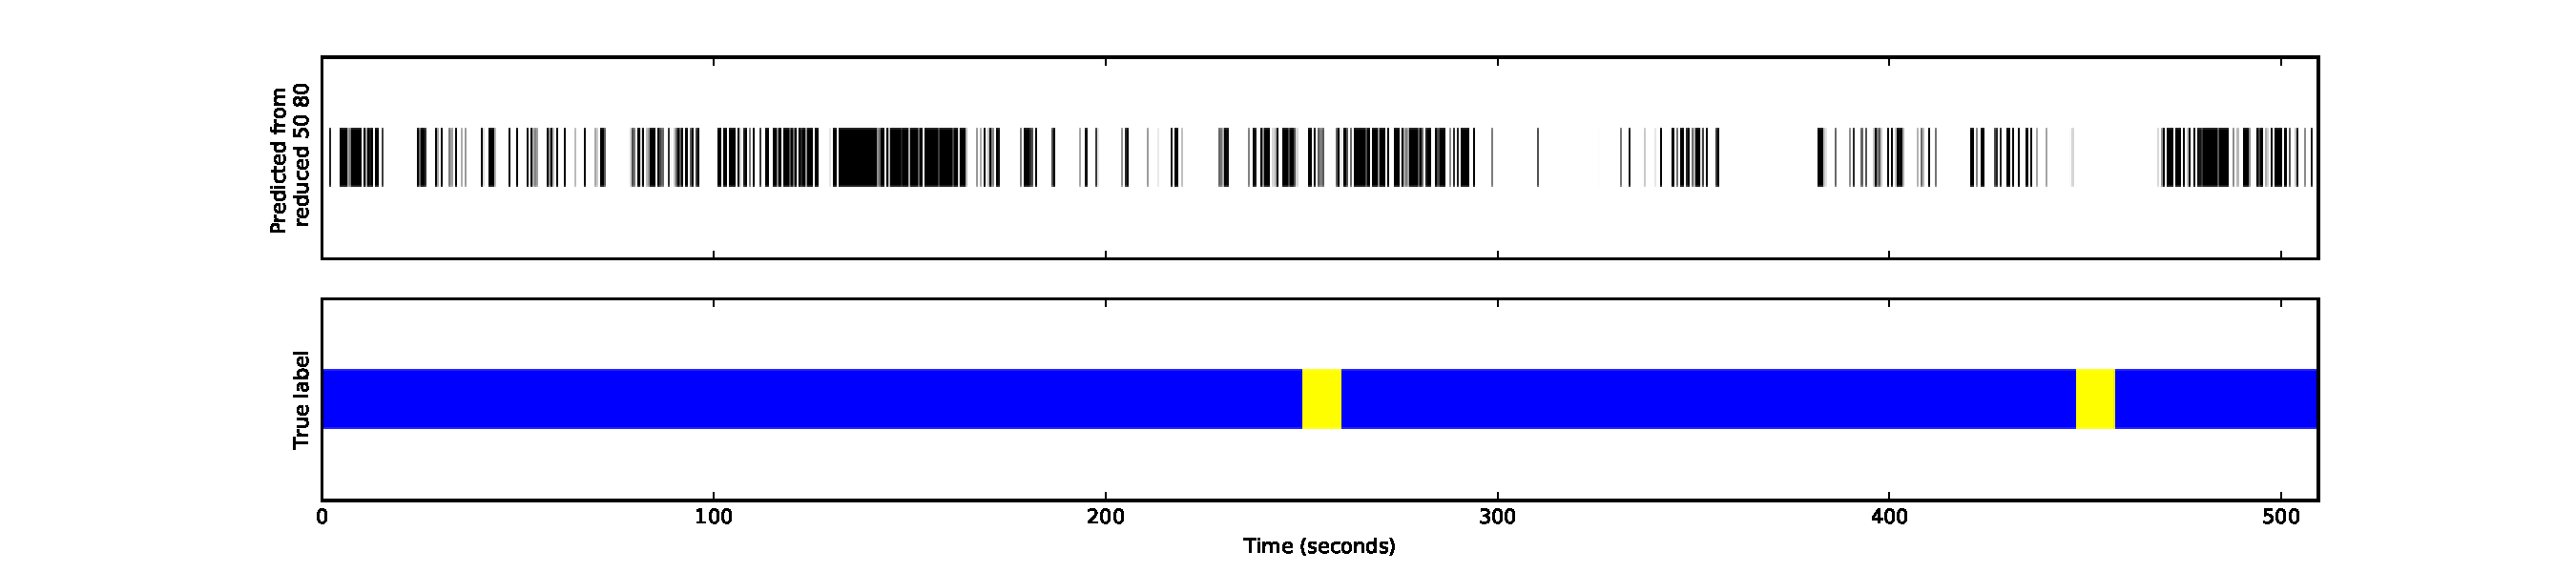
\includegraphics[width=\linewidth]{figures/strip_visual.pdf}
	\caption{Time strips that show the epilepsy time track and the results of the respective clustering done on the Sugihara Causality graphs from those time windows. Blue corresponds to true non-epileptic state; yellow to true epileptic state; white to predicted epileptic state; and black to predicted non-epileptic state. There are only two clusters in the top bar. The clustering results does not show any correlation with the actual epilepsy induction time series.}
	\label{fig:strip_visual}
\end{figure}
% In this section, you will need to provide some form of visualization that emphasizes an important quality about the project. It is much more free-form, but should reasonably support a significant result or characteristic about the problem that you want to discuss. Questions to ask yourself when writing this section:

% Have you visualized a relevant or important quality about the problem, dataset, input data, or results?
% Is the visualization thoroughly analyzed and discussed?
% If a plot is provided, are the axes, title, and datum clearly defined?


\subsection{Reflection}
This project transformed 32 EEG electrode signals into 12 regional neuronal activity signals, and created a (theoretical) communication network from those signals using Sugihara Causality. These communication graphs were analyzed by unsupervised learning using the Gaussian Mixture model for the goal of gaining some insight into the epileptic state, and test whether unsupervised clustering is able to discriminate between brain states from the communication networks. From our initial results, it is clear that our approach is not successful in distinguishing brain states in a rat's brain. However, the ground work has been laid for future explorations in the topic of communication networks in the brain. 

% In this section, you will summarize the entire end-to-end problem solution and discuss one or two particular aspects of the project you found interesting or difficult. You are expected to reflect on the project as a whole to show that you have a firm understanding of the entire process employed in your work. Questions to ask yourself when writing this section:

% Have you thoroughly summarized the entire process you used for this project?
% Were there any interesting aspects of the project?
% Were there any difficult aspects of the project?
% Does the final model and solution fit your expectations for the problem, and should it be used in a general setting to solve these types of problems?

\subsection{Improvement}
Since various improvements can be made to this work, we break it down by stage of implementation.
\subsubsection{Methods}
It would have been enriching to our knowledge of our true labels if we had access to exactly what the rat was doing during the experiment. A video capture of the rat, or recorded structured interventions to the rat's behavior could have provided more opportunity to label the data with ground truth. For example, we could have shone light into the rat's eyes, and recorded that as a separate brain state; we could have put the rat on a hamster wheel and recorded his running as a separate brain state; eating food could be a brain state; and sleeping is another possible brain state. All these interventions to the rat's environment could enable us to gain more labels rather than the simple epilepsy, non-epilepsy labeling system we worked with. Although this complicates our approach, it would allow us access to better scoring metrics other than the silhouette and Calinksy-Harabaz scores, where the labels have to be known.

\subsubsection{Data Processing}
Apart from collecting the data and applying Sugihara Causality on the dataset (which took 2 days), calculating the current source density using kCSD was by far the most time consuming process. Even though we do not discuss the details of how that was done in this project (we provide already processed kCSD data), it would have been nice to see a GPU implementation of the kCSD, which took advantage of CPU parallelism but not GPU parallelism. This would massively improve the speed of the implementation and allow for testing more various approaches in the Sugihara Causality step. 

\subsubsection{Cluster Scoring with Higher Dimensions}
Due to the high dimensionality of the dataset we worked with, it was difficult to visually measure how well the clustering with different number of clusters took place. Beyond three dimensions, it is impossible to visualize the dataset with labels, and although the PCA reduction resulted in a greatly reduced dimensional feature, it was not enough to allow us to visualize the clusters visually.



% In this section, you will need to provide discussion as to how one aspect of the implementation you designed could be improved. As an example, consider ways your implementation can be made more general, and what would need to be modified. You do not need to make this improvement, but the potential solutions resulting from these changes are considered and compared/contrasted to your current solution. Questions to ask yourself when writing this section:

% Are there further improvements that could be made on the algorithms or techniques you used in this project?
% Were there algorithms or techniques you researched that you did not know how to implement, but would consider using if you knew how?
% If you used your final solution as the new benchmark, do you think an even better solution exists?










% \thispagestyle{empty}
% \cleardoublepage

% \tableofcontents

% \thispagestyle{empty}
% \cleardoublepage


\section*{Acknowledgment}
Special thanks goes to Dr. Somogivari and Dorrottya R. from Winger RCP, Budapest for providing the neuronal data used in this paper. Furthermore, Dr. Peter Erdi is thanked for his patient guidance of this research topic which was instrumental for the production of this paper.
\balance
\bibliographystyle{IEEEtran}
\bibliography{IEEEabrv,main.bib}
\end{document}

